\hypertarget{opencvsaving.cpp-example}{
\subsection{opencvsaving.cpp}
}
\begin{DoxyAuthor}{Author}
Rosen Diankov
\end{DoxyAuthor}
 
\begin{DoxyImage}
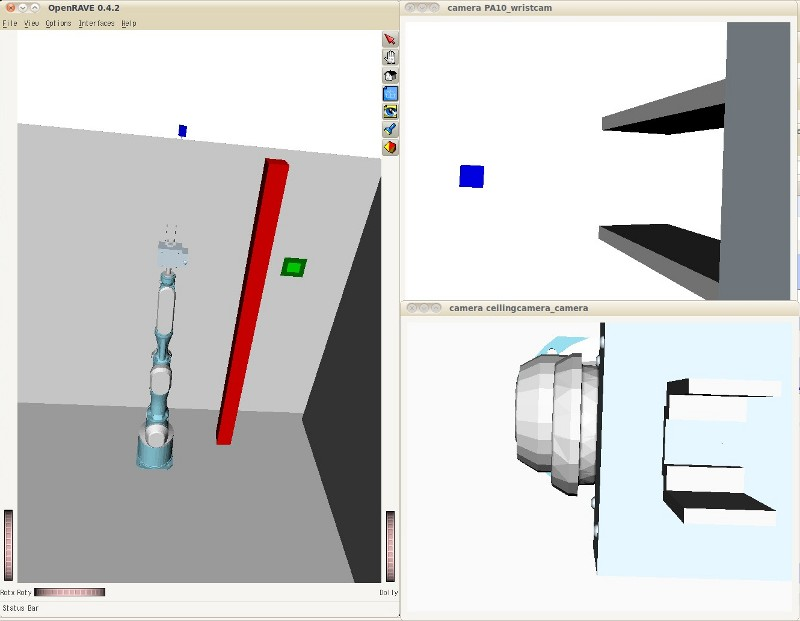
\includegraphics[width=10cm]{cppexample_opencvsaving.jpg}
\caption{OpenRAVE Environment with two cameras.}
\end{DoxyImage}


This example shows how to enable all cameras loaded in an environment and convert their image data to the OpenCV IplImage structure. Then cvSaveImage is called for each image.


\begin{DoxyCodeInclude}

#include <openrave-core.h>
#include <vector>
#include <boost/thread/thread.hpp>
#include <boost/bind.hpp>
#include <opencv/cv.h>
#include <opencv/highgui.h>

#ifdef _WIN32
#define WIN32_LEAN_AND_MEAN
#include <winsock2.h>
#define usleep(micro) Sleep(micro/1000)
#endif

using namespace OpenRAVE;
using namespace std;

void SetViewer(EnvironmentBasePtr penv, const string& viewername)
{
    ViewerBasePtr viewer = RaveCreateViewer(penv,viewername);
    BOOST_ASSERT(!!viewer);

    // attach it to the environment:
    penv->AddViewer(viewer);

    // finally you call the viewer's infinite loop (this is why you need a separa
      te thread) :
    bool showgui = true;
    viewer->main(showgui);
}

class OpenRAVECamera
{
public:
    OpenRAVECamera(SensorBasePtr psensor)
    {
        pcamera=psensor;
        pdata = boost::static_pointer_cast<SensorBase::CameraSensorData>(pcamera-
      >CreateSensorData(SensorBase::ST_Camera));
        geom = *boost::static_pointer_cast<SensorBase::CameraGeomData>(pcamera->G
      etSensorGeometry(SensorBase::ST_Camera));
        img = cvCreateImage(cvSize(geom.width,geom.height),IPL_DEPTH_8U,3);
    }
    virtual ~OpenRAVECamera() {
        cvReleaseImage(&img);
    }

    SensorBasePtr pcamera;
    SensorBase::CameraGeomData geom;
    boost::shared_ptr<SensorBase::CameraSensorData> pdata;
    IplImage* img;
};

int main(int argc, char ** argv)
{
    RaveInitialize(true); // start openrave core
    EnvironmentBasePtr penv = RaveCreateEnvironment(); // create the main environ
      ment
    boost::thread thviewer(boost::bind(SetViewer,penv,"qtcoin"));
    penv->Load("data/pa10calib_envcamera.env.xml");

    std::vector<RobotBasePtr> vrobots;
    penv->GetRobots(vrobots);
    if( vrobots.size() > 0 ) {
        RAVELOG_INFO("moving the robot a little\n");
        Transform t = vrobots.at(0)->GetTransform();
        t.trans.x += 0.6;
        vrobots.at(0)->SetTransform(t);
    }

    // extract all the cameras
    std::vector<SensorBasePtr> allsensors;
    penv->GetSensors(allsensors);
    std::vector< boost::shared_ptr<OpenRAVECamera> > vcameras;
    for( std::vector<SensorBasePtr>::iterator itsensor = allsensors.begin(); itse
      nsor != allsensors.end(); ++itsensor) {
        if( (*itsensor)->Supports(SensorBase::ST_Camera) ) {
            (*itsensor)->Configure(SensorBase::CC_PowerOn);
            (*itsensor)->Configure(SensorBase::CC_RenderDataOn);
            vcameras.push_back(boost::shared_ptr<OpenRAVECamera>(new OpenRAVECame
      ra(*itsensor)));
        }
    }
    while(1) {
        // read the camera data and save the image
        for(size_t icamera = 0; icamera < vcameras.size(); ++icamera) {
            vcameras[icamera]->pcamera->GetSensorData(vcameras[icamera]->pdata);
            if( vcameras[icamera]->pdata->vimagedata.size() > 0 ) {
                char* imageData = vcameras[icamera]->img->imageData;
                uint8_t* src = &vcameras[icamera]->pdata->vimagedata.at(0);
                for(int i=0; i < vcameras[icamera]->geom.height; i++, imageData +
      = vcameras[icamera]->img->widthStep, src += 3*vcameras[icamera]->geom.width) {
                    for(int j=0; j<vcameras[icamera]->geom.width; j++) {
                        imageData[3*j] = src[3*j];
                        imageData[3*j+1] = src[3*j+1];
                        imageData[3*j+2] = src[3*j+2];
                    }
                }
                string filename = str(boost::format("camera%d.jpg")%icamera);
                RAVELOG_INFO(str(boost::format("saving image %s")%filename));
                cvSaveImage(filename.c_str(),vcameras[icamera]->img);
            }
        }
        usleep(200000);
    }

    return 0;
}
\end{DoxyCodeInclude}
 